\documentclass[twocolumn]{article}
\usepackage[a4paper, total={18cm, 26cm}]{geometry}
\usepackage[utf8]{inputenc}

% Support for easy cross-referencing
\usepackage{graphicx}
\usepackage{amsmath}
\usepackage{multirow}
\usepackage[capitalize]{cleveref}
\crefname{section}{Sec.}{Secs.}
\Crefname{section}{Section}{Sections}
\Crefname{table}{Table}{Tables}
\crefname{table}{Tab.}{Tabs.}
\date{}
\title{}
\author{}


\begin{document}
\noindent with ${k}_{s}$ being the spatially-varying specular gain and $\alpha$ a
global roughness blend factor for the Blinn-Phong distri-
bution term D of the 2-lobe mix (${D}_{12}$ and ${D}_{48}$ ) suggested
by [37]. G denotes the geometry term of the Cook-Torrance
BRDF model. We use Shlick’s approximation [40] for the
Fresnel term F :
$$
F({\bf n},\omega) = {F}_{0} + (1 - {F}_{0})(1-{{\bf n}}^\intercal T \omega)^5.
$$

To model the skin’s diffuse response, we implement the
BRDF model proposed by Ashikhmin and Shirley [2, 3],
that accounts for the fact that a portion of the light has al-
ready scattered before penetrating the skin surface:
$$
{f}_{a}({\bf x},\omega) = \frac{28{k}_{d}({\bf x})}{23\pi}(1 - {F}_{0})(1 - (1 - \frac{{\bf n}^\intercal T \omega}{2})^5)^2,
$$

where ${F}_{0}$ = 0.04 is the reflectance of the skin at normal in-
cidence. Indirect light bouncing from the capture environ-
ment and on the captured face itself might have a significant
contribution to pixel intensity at grazing angles, so we also
add a Fresnel-modulated ambient term to our BRDF $f$ :
$$
{f}_{a}({\bf x},\omega) = {k}_{a}({\bf x})(1 - (1 - {F}_{0})(1 - (1 - \frac{{\bf n}^\intercal T \omega}{2})^5)^2),
$$
with an ambient map ${k}_{a}$ which is regularized to be smooth
via a total variation loss and close to zero.

\indent Note that using a diffuse scattering model for the op-
timization is compatible with state-of-the-art physically-
based subsurface scattering skin shading [5, 49], as shown
in Figure 1. Production-ready subsurface scattering models
typically include an albedo inversion stage, which takes a
diffuse albedo as input, and converts it to extinction coeffi-
cients for the volume rendering random walk.

\subsection*{3.4 Optimization}\label{3.4}

The objective of the photometric optimization step is to
minimize the difference between rendered images \^I and
color-corrected target images \textit{I}:

$$
\mathcal{L}(\^I,I) =  |W \cdot (\^I - I)|,
$$

with $\^I = \mathcal{M} \cdot {L}_{o}$ , where $\mathcal{M}$ is the pre-computed light at-
tenuation map, that accounts for uneven light distribution
in different directions. We apply a per-pixel loss weight
W based on the respective mip level and the angle between
viewing direction and normal ${\bf n}^\intercal T \omega$ to improve sharpness.
Specifically, to ensure that distant or grazing angle observa-
tions do not blur the resulting textures, for each pixel that is
projected from the target image to texture space, we calcu-
late which mip level $l$ would need to be looked up in classi-
cal forward rendering. W is set to $({\bf n}^\intercal T \omega)(1 - l)$ if the pixel
corresponds to a mip level below 1, and zero otherwise.

\begin{table}[]
    \centering
    \begin{tabular}{c c c c}
         \textbf{Method} &  \textbf{PSNR} & \textbf{SSIM} & \textbf{LPIPS}\\ \hline
         NLT & 31.51 & \textbf{0.96} & 0.11 \\
         NextFace & 22.85 & 0.89 & 0.31 \\\hline
         Ours & \textbf{32.37} & \textbf{0.96} & \textbf{0.10} \\\hline
    \end{tabular}
    \caption{We compare our method to NLT and NextFace on validation frames over 10 different subjects}
    \label{tab:Table 1}
\end{table}


\newpage
\indent We optimize $\mathcal{L}(\^I,I)$ in two steps, using a coarse-to-fine
optimization strategy in each. In the first step, we only use
the cross-polarized images to optimize the spatially-varying
diffuse albedo texture ${k}_{d}({\bf x})$ and an initial tangent-space
normal map $n({\bf x})$, while assuming ${f}_{s}(\cdot)$ = 0 for the specu-
lar term. In the second step, we fix the diffuse texture and
optimize for specular gain ${k}_{s}({\bf x})$, specular roughness α, and
the final normal map $n({\bf x})$. To account for potentially dif-
ferent light attenuation in the cross and parallel-polarized
filter settings, we also optimize per-channel scaling factors
for the diffuse texture. The optimization is performed en-
tirely in texture space. In each step, we employ a four-level
coarse-to-fine optimization strategy, starting with a texture
resolution of 512 × 512, and increasing the size by a fac-
tor of two after convergence of each level, up to the final
resolution of 4096 × 4096.


We implement our optimization framework in PyTorch,
using nvdiffrast [24] as our differentiable renderer. We op-
timize on batches of 4 images, using Adam with an ini-
tial learning rate ${lr}_{0} = 10^{-3}$ for all parameters at the
beginning of every coarse-to-fine step, and updating it to
$lr = {lr}_{0} \cdot 10^{-0.001t}$ in every iteration $t$. We scale the
FLAME mesh to unit size and set the light intensity to 10.
The total optimization time is about 90 minutes.

\section*{4. Results}
In this section, we present texture reconstruction and ren-
dering results on several subjects. Figure 5 shows the tex-
ture reconstruction on several actors of different ethnicity.
Our method is able to reconstruct pore-level detail in the
diffuse, specular and normal maps. Further, we evaluate the
quality of our reconstructed textures by rendering the mesh
from novel views and under novel illumination. Figure 6
shows that our method faithfully reconstructs the skin’s ap-
pearance under novel views and lighting. \textit{We recommend
the reader to use the zoom function of the PDF viewer to
inspect the details}.

\textbf{Comparison to state of the art.} We perform both a qualita-
tive and quantitative evaluation of our method and compare
to state-of-the-art methods for relighting and texture recon-
struction. During optimization, we hold out a validation
frame on which we compute image metrics.

\indent \textit{Neural Light Transport.} Neural Light Transport [55]
is a deep learning-based method that takes as input pre-

\newpage
\begin{figure}
    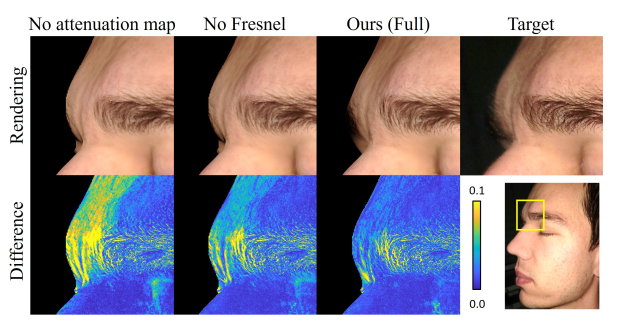
\includegraphics{image/image1.png}
    \caption{Ignoring the angle-dependent flashlight attenuation or
the Fresnel effect leads to an incorrect diffuse map reconstruction,
that can no longer reproduce the shading from all views. We ac-
count for both to closely match the target data.}
    \label{fig:Figure 8}
\end{figure}

\begin{figure}
    \includegraphics{image/image2.png}
    \caption{We run a joint optimization of all textures and compare a
purely diffuse render to our full approach. As visible in the figure,
optimizing the textures jointly will leak specular and normal map
information into the diffuse texture.}
    \label{fig:Figure 9}
\end{figure}

skin’s diffuse response at all angles. In Figure 9, we show
that optimizing textures without cross-polarization will leak
specular information into the diffuse texture.
\newline

\noindent \textbf{Coarse-to-fine optimization and mipmapping.} The pix-
els of the target images may have different footprints in
uv-space, depending on distance and angle between the
camera and the surface. Weighting the loss of each pixel
equally would lead to blurriness in the reconstructed tex-
tures. Optimizing coarse-to-fine, where at each resolution
we use only pixels with the corresponding uv-space foot-
print, helps us reconstruct additional detail in the textures.
Figure 10 shows a comparison between our full approach
and one where we directly optimize the highest resolution
texture. We additionally show the decrease in quality when
optimizing only on the video frames (w/o photographs).

\newline

\noindent \textbf{Runtime and memory consumption.} Including one hour
that is spent on MVS, our method takes about 2.5h to re-
construct a person’s face. The photo-metric skin texture
reconstruction takes about 90 minutes on an Nvidia RTX
A6000. We reconstruct the facial geometry with Metashape
using an average of 420 video frames and 70 photographs.
At a texture resolution of 4096 × 4096 and target image
\maketitle
{\small
\bibliographystyle{}
\bibliography{r}
}

\end{document}
